\documentclass[12pt, a4paper, twoside]{article}

%% Preamble
\usepackage{tfm-style-guide}
\usepackage{blindtext}
\usepackage{graphicx}
\usepackage{relsize}
\usepackage{txfonts}
\usepackage{amssymb}
\usepackage{float}
\usepackage{titlesec}
\usepackage{float}
\usepackage{listings, lstautogobble}
\usepackage{dsfont}
\usepackage[OT1]{fontenc}
% \usepackage{amsmath}
\usepackage[backend=biber, sorting=none]{biblatex}
\addbibresource{bibliography.bib}

\definecolor{RoyalBlue}{cmyk}{1, 0.50, 0, 0}

\lstset{language=C,
keywordstyle=\color{RoyalBlue},
basicstyle=\scriptsize\ttfamily,
commentstyle=\ttfamily\itshape\color{gray},
stringstyle=\ttfamily,
showstringspaces=false,
breaklines=true,
frameround=ffff,
frame=single,
rulecolor=\color{black},
autogobble=true
}



\begin{document}
\cleardoublepage

%% Abstract English
\selectlanguage{english}
\begin{abstract}
	
	\bfseries{\large{Keywords:}} Static Application Security Testing, Large Language Models, C programming language, False Positives
\end{abstract}

\newpage

%% Abstract Spanish
\selectlanguage{spanish}
\begin{abstract}
	\bfseries{\large{Keywords:}} Analizador de código estático, Modelo extenso de lenguaje, Lenguaje de programación C, Falsos positivos
\end{abstract}


\tableofcontents	

\listoffigures

\section{Introducción}
El lenguaje de programación C es uno de los lenguajes más populares en la industria de desarrollo de software. Este lenguaje adquiere una notable presencia en sistemas en los que se necesita del acceso a bajo nivel al hardware, la eficiencia temporal y el control explícito de los recursos. Originalmente, C se planteo como un lenguaje de programación de sistemas para la familia de sistemas operativos tipo UNIX,  caracterizado técnicamente como un lenguaje liviano, de propósito general y portable \cite{seacord-2013}. Una gran cantidad de aplicaciones de alto rendimiento y sistemas críticos se implementan en C y continúan en soporte.

Sin embargo, las características que popularizaron a C también son el fondo detrás de una gestión insegura de la memoria intrínseca al lenguaje. Esta gestión insegura propicia la aparición de errores en el manejo de la memoria, que, además de ser difíciles de detectar, constituyen una de las superficies de ataque más persistentes en los lenguajes de programación \textit{memory-unsafe}.

Los lenguajes de programación \textit{memory-unsafe} no cuentan, por defecto, con mecanismos de prevención de errores comunes de programación relacionados con la libertad en el acceso a memoria. Bajo esta libertad, el programador gestiona manualmente la memoria, pero esta libertad conlleva la aparición de distintos tipos de vulnerabilidades, entre las que figuran los desbordamientos de pila, las filtraciones de memoria y la corrupción de memoria.

Concretamente, las vulnerabilidades de corrupción de memoria constituyen el tipo de vulnerabilidad más frecuente. La sobre-escritura de metadatos del montículo, los punteros colgantes, las lecturas de memoria no inicializada, las liberaciones inválidas de memoria o la doble liberación de memoria son debilidades reconocidas por investigadores de seguridad y cuentan con sus respectivas técnicas de protección para abordarlas \cite{moghadam-2024}.

Cada una de las vulnerabilidades anteriormente mencionadas se recogen en la Common Weakness Enumeration (CWE), por lo que hacemos énfasis en que las fallas que se encuentran en programas escritos en C no son errores individuales aislados, sino que son consecuencia del diseño estructural del lenguaje.

A la vista de este escenario, la detección de debilidades supone una necesidad con objeto de asegurar la calidad y diseñar software seguro. La literatura sobre el análisis de programas señala una reducción en el coste de corrección de vulnerabilidades si se detectan tempranamente. De hecho, facilita la implementación de prácticas de seguridad <<\textit{shift-left}>> e intervenir antes de que los defectos lleguen a la etapa de despliegue o de explotación \cite{cifuentes-2023}.

Los analizadores de código estático son herramientas que permiten la detección de vulnerabilidades en el código fuente a partir de la detección de patrones. Son herramientas de referencia en la industria de desarrollo software, por ejemplo en las canalizaciones de integración continua, dado que permiten identificar estas vulnerabilidades en las fases tempranas del ciclo de vida del software. Por el contrario, hay estudios empíricos que muestran sus limitaciones en la precisión, cobertura, explicabilidad y unas altas tasas de positivos en sus reportajes \cite{aloraini-2019}. Por lo tanto, detectar estas vulnerabilidades asegurando una alta fiabilidad y utilidad sigue siendo un problema abierto.

\section{Estado del arte}
En el contexto de este trabajo profundizaremos en el análisis de vulnerabilidades relacionadas con la pila de llamadas, también llamada pila o \textit{call stack} y el montículo, también llamado \textit{heap}, en el lenguaje C. Ambas son dos regiones de memoria relevantes en la estructura de los programas en tiempo de ejecución.
% Tanto en C como en C++ se delega en el programador la gestión de la memoria del programa, de forma los programadores interactúan directa o indirectamente con estas regiones de datos \cite{hertz-2005}.
Expondremos el funcionamiento de ambas, y posteriormente explicaremos sus  debilidades.

\subsection{El funcionamiento de la pila de llamadas}
En la pila de llamadas (\textit{stack call}) se almacenan los datos relativos a las subrutinas de un programa. Cuando se invoca una subrutina, se crea en la pila un nuevo marco \textit{stack frame}, que contiene sus parámetros, la dirección de retorno y sus variables locales. Al finalizar la subrutina, su marco se libera.

La pila sigue una estrategia LIFO (\textit{last in, first out}): el último marco en crearse es el primero en destruirse. Por ello, las subrutinas más anidadas (las llamadas más recientes) son las últimas en asignarse pero las primeras en liberarse, de forma análoga a una pila de libros donde solo se puede retirar el libro de la cima.

%La estrategia de gestión de datos que implementa la pila se basa en que la primera entrada que se desaloja es la última que se añadió, dicho de otra forma, la pila sigue la estrategia LIFO. Es por esto que conforme se ejecutan las subrutinas en un programa, las primeras que se alojan son las que se encuentran anidadas dentro de esta, y, consecuentemente, serán las las primeras que se liberen en la pila. Es por ello que, análogamente, su funcionamiento se asemeja al de una pila de libros, apilándose estos uno encima de otro y retirándolos desde el que se encuentra más arriba al que esta más abajo.

La gestión de la pila se realiza mediante un puntero de pila. Al insertar un nuevo marco, el puntero se desplaza hasta el tope de dicho marco. Y al salir, el puntero retrocede hasta el tope del marco anterior (o al límite inicial si la pila queda vacía). Estos movimientos son automáticos y el programador no tiene control directo sobre ellos.

%El mecanismo de alojamiento en la pila se basa en el desplazamiento de un puntero de memoria. Por cada marco de pila que se inserta, el puntero se mueve hasta el final del marco. En la salida del marco de pila ocurre a la inversa, el puntero se desplaza al final del marco anterior, o en su defecto del limite inicial de la pila. Ambos mecanismos son automáticos, de forma que sobre ellos no tiene control directo el programador.


\subsection{El funcionamiento del montículo (\textit{heap})}
El montículo (heap) es una región de memoria dinámica; es decir, los datos almacenados en él se asignan durante el tiempo de ejecución del programa. A diferencia de la pila, los datos del montículo deben gestionarse manualmente. 

La gestión manual de la memoria comprende dos operaciones fundamentales: la petición y la liberación de bloques de memoria. Para solicitar un bloque de un número especifico de bytes, se emplean las funciones \texttt{malloc()} o \texttt{calloc()}, que devuelven la dirección de memoria del bloque asignado.
La liberación se realiza mediante la función \texttt{free()}, a la que se proporciona como argumento la dirección del bloque que se desea liberar. 
% Ambas operaciones interactúan con el administrador de memoria del entorno de ejecución, el cual puede solicitar memoria al sistema operativo en bloques mayores para optimizar el rendimiento \cite{amini-2019}.

Al delegar la gestión de la memoria en el programador, los errores aparecen con una frecuencia mucho mayor. Uno de los más característicos son las \textbf{fugas de memoria} (memory leaks), que ocurren cuando no se libera un bloque de memoria tras cumplir su utilidad. En casos severos, puede llevar al agotamiento de los recursos (especialmente en dispositivos con capacidades limitadas), lo que puede derivar en una denegación de servicio \cite{cal-2002}.

\subsection{Organización de la memoria interna de un proceso}
Dentro de un proceso, la pila y el montículo comparten la misma región de memoria, con la particularidad de que ambas crecen en direcciones opuestas. Por un lado, la pila tiene un límite de tamaño impuesto por el sistema: en Linux puede crecer hasta 8 MB, mientras que en Windows el limite es típico es de 1 MB. En cambio, montículo puede crecer hasta agotar la memoria virtual disponible. En la figura \ref{fig:estructura-memoria-proceso} se observa esta región compartida dentro de la estructura de memoria un proceso.

\begin{figure}[htpb]
	\centering
	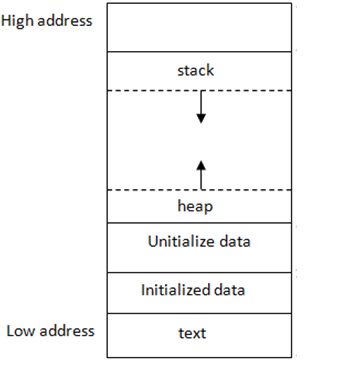
\includegraphics[width=0.4\textwidth]{images/estructura-memoria-proceso.png}
	\caption{Estructura de memoria de un proceso C/C++. Extraída de \cite{chen-guo-cs225}}
	\label{fig:estructura-memoria-proceso}
\end{figure}


%Por otra parte, en el segmento de datos, la pila comparte la misma región de memoria que el montículo; con la particularidad de que los punteros de direcciones de ambos crecen en sentidos opuestos. En la mayoría de arquitecturas de computadores, se decide por convención que la pila crece decrementando el puntero mientras que el montículo lo hace incrementándolo. En la figura \ref{fig:estructura-memoria-proceso} se observa la estructura en memoria que ambas regiones comparten el mismo espacio de direcciones.

%Puesto que ambas estructuras coexisten en la misma región de memoria, existe un limite de tamaño al cual pueden crecer la pila, no teniendo el montículo esa restricción. Esta diferencia de restricciones la expondremos más a fondo en la sección dedicada al montículo. Por lo pronto, la pila de llamadas tiene un tamaño nominal específico según la plataforma de ejecución \cite{avd-2009}, y dada esta restricción se desprende el error por \textbf{desbordamiento de la pila}. Su aparición se da cuando en un programa se usa más memoria de la que tiene disponible en la pila de llamadas. En otros términos, ocurre cuando el puntero de la pila de llamadas excede el tamaño límite.

\subsection{CWEs de la pila de llamadas}
\label{sec:cwe-stack}
Las debilidades que vamos a tratar se recogen en el catalogo CWE (\textit{Common Weakness Enumeration}) de MITRE, el cual contiene fallos estandarizados conocidos por causar vulnerabilidades. Tanto la gestión de la pila, como la región de memoria en sí, tienen asociadas múltiples debilidades, de forma que en este artículo recogemos las ocho más relevantes para el propósito de nuestro estudio.

\begin{itemize}
	\item \textbf{CWE-121: Desbordamiento del búfer en la pila}. Ocurre cuando se escribe más allá de los límites de un búfer asignado en la pila. Pudiendo corromper datos en marcos adyacentes, como variables o direcciones de retorno, y potencialmente permitir la ejecución de código arbitrario \cite{mitre-cwe-121}.
	%En la figura \ref{} puede verse 
	
	\item \textbf{CWE-562: Devolución de puntero de pila}. Ocurre cuando una función devuelve un puntero a una variable local. Al finalizar la ejecución de dicha función, su marco de pila se destruye y todas las referencia a las variables locales que contenía quedan invalidadas. Por tanto, el puntero devuelto apunta a una región de memoria ya desasignada, cuyo uso posterior constituye un comportamiento indefinido y potencialmente explotable \cite{mitre-cwe-562}.
	
	\item \textbf{CWE-628: Llamada a función con argumentos especificados incorrectamente}. Constituye una categoría base de vulnerabilidades de las cual se desglosan varias vulnerabilidades hijas. Entre las vulnerabilidades hijas podemos encontrar tres específicas de la pila de llamadas.
	\subitem \textbf{CWE-683: Llamada a función con argumentos en orden incorrecto}.
	\subitem \textbf{CWE-685: Llamada a función con número incorrecto de argumentos}.
	\subitem \textbf{CWE-688: Llamada a función con una variable o referencia incorrecta como argumento}.
	
	\item \textbf{CWE-674: Recursión no controlada}. Se da en el caso de una función recursiva la cual carece de un caso base adecuado o de un límite en su profundidad, lo que lleva a un consumo masivo de memoria de pila (\textit{stack memory}) y al agotamiento de su espacio.
	
	%\item \textbf{CWE-789: Asignación de memoria con tamaño excesivo}. Ocurre cuando se asignan datos en memoria basándose en un tamaño proporcionado por un atacante, lo que puede llevar a un agotamiento de la misma. Puede ocurrir cuando los datos se obtienen de orígenes que no son de confianza y sobre los que no se comprueban los límites esperados \cite{mitre-cwe-789}.
	
	\item \textbf{CWE-835: Bucle con condición de salida inalcanzable}. Se da cuando el programa entra en un bucle infinito, lo que lleva a un agotamiento de la pila. Un ejemplo puede ser un bucle \texttt{while(true)} sin una instrucción \texttt{break}.
	
	% \item \textbf{CWE-1325: Control inadecuado en la asignación de memoria secuencial}. Ocurre cuando no se controla el espacio consumido al asignar variables con la función \texttt{alloca()}, la cual almacena los datos directamente en el marco de pila \cite{mitre-cwe-1325}.
\end{itemize}
% Las debilidades recogidas en el catalogo CWE son fallos estandarizados conocidos por causar vulnerabilidades. En este apartado detallamos 5 fallos asociados a la pila de llamadas.


%\subsection{Causas del desbordamiento de pila}
%Generalmente, los desbordamientos de pila pueden atribuirse a dos causas, aquellos que tienen que se deben a función recursiva, que debido a la cantidad de datos que aloja con sus llamadas agota el espacio de la pila; y aquellos se dan al intentar almacenar variables excesivamente grandes en la pila.

%% Esto es una mierda
% La recursión infinita carece de caso base, sabemos que tecnicamente, al no finalizar nunca, 
%Las funciones recursivas son aquellas funciones que se llaman a si mismas dentro de su propio código, estas funciones para evitar llamadas infinitas cuentan con un caso base, que es una condición que al cumplirse detiene las llamadas recursivas. Aunque hacemos enfasís 

%Un desbordamiento de pila puede deberse en una función recurvis. El primero es que haya una profundidad excesiva de llamadas, aunque todos los marcos contengan la misma cantidad de datos; y segundo, que haya un crecimiento en el tamaño de los marcos con la profundidad (por ejemplo, cuando cada marco nuevo contiene estructuras de datos de mayor tamaño que las anteriores), acelerándose así el ritmo de consumo de la pila. En ambos casos, tanto en funciones recursivas con casos base lejanos, como con marcos de tamaño creciente, se puede producir un desbordamiento. En la figura \ref{fig:contenido-pila-programa-recursivo} puede verse un ejemplo de funciones recursivas en las que el tamaño del marco crece conforme aumenta la profundidad.

%Obviando la recursión infinita, dado que no es posible en un sistema con recursos finitos, nos centraremos en la recursión finita. En estos terminos, un desbordamiento de pila puede darse si el ritmo de crecimiento de la pila se acelera conforme aumenta el nivel de profundidad; dicho de otro modo, conforme se insertan nuevos marcos, estos contienen cada vez más datos que el anterior. Las funciones recursivas de gran profundidad pueden llevar a un desbordamiento de pila. Un ejemplo de este tipo de comportamientos puede verse en la figura \ref{fig:contenido-pila-programa-recursivo}.

%\begin{figure}[htpb]
%	\centering
%	\begin{minipage}{.45\columnwidth}
%		\begin{lstlisting}
%			int pow(int base, int exp) {
%				if (exp > 0) {
%					return base * pow(base, exp - 1);
%				} else {
%					return 1;
%				}
%			}	
%		\end{lstlisting}
%	\end{minipage}
%	\hfill
%	\begin{minipage}{.45\columnwidth}
%		\begin{lstlisting}
%			pow(5, 4)
%			5 * pow(5, 3)
%			5 * (5 * pow(5, 2))
%			5 * (5 * (5 * pow(5, 1)))
%			5 * (5 * (5 * (5 * pow(5, 0))))
%			5 * (5 * (5 * (5 * 1)))
%			625
%		\end{lstlisting}
%	\end{minipage}
%	\caption{A la izquierda se tiene el código fuente, a la derecha, el contenido de la pila en el nivel más profundo de recursión. En este caso, el calculo se expande según se profundiza. En situaciones de recursividad muy profunda, aumenta el riesgo de desbordamiento de pila por agotamiento de espacio. Ejemplo extraído de Wikipedia \cite{enwiki:1351011401}.}
%	\label{fig:contenido-pila-programa-recursivo}
%\end{figure}

%El tamaño de las variables se calcula en tiempo de compilación. Las colecciones de datos excesivamente grandes pueden provocar errores por agotamiento del espacio disponible. En la figura se dispone de un ejemplo susceptible de agotar el espacio de la pila.

\subsection{CWEs del montículo}
\label{sec:cwe-heap}
Hay muchos CWEs recogidos que pueden asociarse al montículo, de forma que para nuestro estudio hemos realizado un listado con sus ocho debilidades más relevantes.

\begin{itemize}
	\item \textbf{CWE-122: Desbordamiento del búfer en el montículo}. Ocurre cuando en un bloque de memoria se escribe escriben más datos de los que caben, de forma que compromete la memoria adyacente y puede derivar en la ejecución de código arbitrario.
	
	%\item \textbf{CWE-193: Error por uno (\textit{Off-by-one error})}. Ocurre cuando la comprobación de una condición lógica se realiza de manera incorrecta, desviándose en una unidad por exceso o defecto. Es frecuente al especificar la condición de salida en bucles iterativos, especialmente en lenguajes de programación cuya indexación comienza en cero en lugar de uno (como es el caso de C/C++) \cite{mitre-cwe-193}.
	
	\item \textbf{CWE-244: Limpieza incorrecta de la memoria antes de su liberación (\textit{Heap Inspection})}.
	Ocurre cuando se libera un bloque de memoria (ya sea explícitamente con \texttt{free()} o implícitamente con \texttt{realloc()}) sin sobrescribir previamente los datos sensibles que contenía. En particular, cuando \texttt{realloc()} necesita reubicar el bloque en una nueva dirección copia su contenido, libera el bloque original y lo deja intacto en el \textit{heap}, aunque inaccesible para el programa. Un atacante que pueda leer volcados de memoria o direcciones liberadas y podría recuperar dichos datos \cite{mitre-cwe-244}.
		
	\item \textbf{CWE-401: Filtraciones de memoria (\textit{Memory Leaks})}.
	Ocurre cuando un bloque de memoria no es liberado después de haber cumplido su función, lo que provoca su acumulación y la imposibilidad de reutilizarlo para otros fines. Cuando el problema persiste de manera sistémica, pueden producirse acumulaciones masivas de memoria. En este escenario, un atacante podría explotar esta debilidad para causar una denegación de servicio (\textit{DoS}, en inglés \textit{Denial of Service}) \cite{mitre-cwe-401}.
	
	\item \textbf{CWE-415: Doble liberación}. Se da cuando se llama a la función \texttt{free()} dos veces sobre la misma dirección de memoria. Esto corrompe la estructura del montículo y puede derivar en fallos inesperados o comportamiento impredecible; en escenarios controlados por un atacante, puede posibilitar ataques de uso tras liberación (\textit{use-after-free}),  que a su vez permiten ejecutar código arbitrario o escalar privilegios \cite{mitre-cwe-415}.
	\subitem \textbf{CWE-416: Uso tras la liberación (\textit{Use-After-Free})}. Ocurre cuando se accede a una región de memoria tras haber sido liberada, sin que el puntero haya sido reasignado o puesto a \texttt{NULL}. Esto provoca que un atacante pueda reutilizar un bloque de memoria liberado, lo que le permite llevar a cabo los ataques previamente descritos \cite{mitre-cwe-416}.
	
	\item \textbf{CWE-476: Desreferencia de puntero nulo}. Ocurre cuando se emplea un puntero bajo la expectativa de que contenga una referencia a una dirección de memoria valida; no obstante, el puntero contiene una referencia a \texttt{NULL}, lo que provoca un fallo en el proceso. En circunstancias excepcionales, cuando \texttt{NULL} apunta a la dirección de memoria \texttt{0x0} y el código privilegiado puede acceder a ella, de forma que es posible leer o escribir en dicha memoria, puede derivar en la ejecución de código arbitrario \cite{mitre-cwe-476}.
	
	\item \textbf{CWE-590: Liberación de memoria no asignada en el montículo}. Ocurre cuando se llama a la función \texttt{free()} con un puntero de memoria no asignado en el montículo. Al liberar un puntero inválido, pueden corromperse el manejo de las estructuras de datos de memoria, lo que provoca fallos en el programa. En el caso de un ataque, un atacante puede usar la función \texttt{free()} para realizar operaciones en memoria de forma que le permitan modificar controles críticos o ejecutar código arbitrario \cite{mitre-cwe-590}.
	
	\item \textbf{CWE-761: Liberación de puntero no situado al inicio del búfer}. Ocurre cuando se llama a la función \texttt{free()} con una dirección de memoria asignada en el montículo, pero que no está al inicio del búfer, lo que provoca un fallo en el programa \cite{mitre-cwe-761}.
\end{itemize}

\subsection{CWEs que afectan tanto a la pila de llamadas como al montículo}
\label{sec:cwe-common}
Las vulnerabilidades recogidas en este apartado se encuentran asociadas tanto a la pila de llamadas como al montículo, por lo que les hemos dedicado un apartado propio. Estas vulnerabilidades comparten una debilidad común, el desbordamiento de búfer, de forma que aprovechan las características de este tipo de vulnerabilidad para explotarla por otros métodos, como veremos a continuación. Recogemos un total de cinco vulnerabilidades más.

\begin{itemize}
\item \textbf{CWE-123: (\textit{Write-what-where})}. Esta vulnerabilidad consiste en cualquier condición que permite a un atacante escribir un valor arbitrario en una dirección de memoria también arbitraria. Este escenario es frecuente en el caso de los desbordamientos de búfer, ya que, al escribir datos que exceden el tamaño del búfer reservado, se pueden sobrescribir posiciones de memoria, lo que permite la ejecución de código arbitrario o la subversión de las medidas de seguridad \cite{mitre-cwe-123}.

\item \textbf{CWE-125: Lectura fuera de los limites del búfer}. Ocurre cuando se realiza una lectura de los datos fuera de las direcciones del búfer. De esta debilidad se desglosan otras dos vulnerabilidades hijas:
\subitem \textbf{CWE-126: Lectura de datos más allá del búfer}
\subitem \textbf{CWE-127: Lectura de datos atrás del búfer}

\item \textbf{CWE 680: Desbordamiento de entero que conduce a desbordamiento de búfer}. Esta vulnerabilidad ocurre cuando, al calcular el tamaño de un búfer, resultado de una operación aritmética supera el valor máximo representable por el tipo entero utilizado. En consecuencia, el búfer asignado tiene una capacidad menor a la esperada, lo que provoca un desbordamiento de búfer la intentar escribir en el más datos de los que puede albergar \cite{mitre-cwe-680}. 
\end{itemize}


\subsection{Modelo extenso de lenguaje ($\textit{Large Language Model}$, $\textit{LLM}$)}
Un modelo extenso de lenguaje es un tipo de modelo de aprendizaje profundo (\textit{deep learning}). En concreto, se trata de un sistema de inteligencia artificial basado en redes neuronales de múltiples capas. Dichos algoritmos emplean cantidades masivas de parámetros y extensos conjuntos de datos de entrenamiento para llevar a cabo tareas de comprensión y predicción de texto \cite{michael-britannica-2026}.

Por consiguiente, estos modelos se inscriben en el ámbito del procesamiento del lenguaje natural (\textit{NLP}, del inglés \textit{Natural Language Processing}). La función principal que desempeñan es la predicción estocástica del siguiente tóken en una secuencia. Este comportamiento se consigue durante el entrenamiento: a partir de los textos con los que se les entrena, aprenden distribuciones de probabilidad sobre secuencias de tókenes, lo que les permite generar texto que sigue los patrones estadísticos observados en los datos. \cite{stryker-2025}

La aplicación de esta funcionalidad se extiende más allá del lenguaje natural, abarcando también el código fuente de programas informáticos. Estos modelos resultan útiles en tareas como la comprensión, generación o explicación de código, la creación de casos de prueba unitarios y la generación de documentación técnica.

\subsection{Transformador ($\textit{Transformer}$)}
El transformador es una arquitectura basada en redes neuronales artificiales con capacidad para procesar secuencias de datos, como textos, imágenes o vídeos. El mecanismo introducido en esta arquitectura que supone novedoso es el mecanismo de auto-atención, en inglés, \textit{Self-Attention Mechanism}.

El mecanismo de auto-atención consiste en la medición de relevancia de cada palabra o elemento respecto al resto dentro de una misma secuencia. Esta medición se representa por medio de tres vectores: Q, K y V. Dónde Q representa la consulta de la palabra en el contexto, K representa el termino sobre el cual se realiza la consulta y V la información semántica asociada a cada clave.

Cada uno de los valores de Q, K y V se extrae de sus respectivas matrices de pesos $W_q$, $W_k$ y $W_v$. De forma que el computo de cada uno de estos vectores se formaliza con las operaciones.
\begin{itemize}
	\item $Q = W_q \cdot x$ 
	\item $K = W_k \cdot x$ 
	\item $V = W_v \cdot x$ 
\end{itemize}
Donde x es un \textit{embedding} de palabras, es decir, una representación del texto en un arreglo númerico.

En la arquitectura del transformador se distinguen dos partes: un codificador y un decodificador. El codificador recibe la entrada y el decodificador genera la salida. El diseño original de esta arquitectura lo propusieron ingenieros de Google para la traducción automática de textos \cite{Vaswani2017-lh}. Sin embargo, esta arquitectura se empleo para otros propósitos, el más singular de ello es su uso en modelos de inteligencia artificial generativa, entre los que se incluyen los \textit{LLM}, por destacar en tareas de <<comprensión>> del lenguaje.

\subsection{Ajuste fino eficiente en parámetros (PEFT)}
También se le denomina como \textit{fine-tuning} eficiente en parámetros. Es una metodología empleada para mejorar el rendimiento de modelos de inteligencia artificial previamente entrenados. Las mejoras de rendimiento pueden consistir en que el modelo ejecute tareas que previamente no podía realizar o que aprenda conjuntos de datos específicos \cite{belcic-2025}.

El ajuste eficiente consiste en un re-entrenamiento de un subconjunto de los parámetros del modelo, de forma el resto de la estructura del modelo se conserva. La preferencia de esta metodología en lugar de un \textit{fine-tuning} tradicional se vincula a las siguientes circunstancias:

Evasión del <<olvido catastrófico>>. Que es la perdida del contexto adquirido en fases de entrenamiento previas, debido a un reajuste de todos los parámetros del modelo durante el proceso de re-entrenamiento o ajuste.

Reducción del riesgo de sobreajuste. El cual es sustancialmente mayor si se induce el modelo a un re-entrenamiento completo, provocando un olvido del contexto con el que se entreno previamente, puesto que se re-ajustan todos los parámetros nuevamente.

Disminución en la demanda de datos. Conforme más parámetros se entrenan, más cantidades de datos se necesitan para disponer al modelo del contexto suficiente para ejecutar la tarea para la cual se entrena.

\subsubsection{Adaptación de bajo Rango (LoRA)}
La adaptación de bajo rango es una técnica empleada para la adaptación de un modelo de inteligencia artificial a nuevos contextos. Exime el re-entreno de potencialmente miles de millones de parámetros, o al menos medio billón de parámetros, agregando matrices de rango bajo que al aplicarlas a las entradas permite ajustar el modelo para obtener resultados específicos según el contexto \cite{noble-2025}.

Estas matrices de rango bajo son las que se ajustan en el proceso de entrenamiento, mientras que el resto de pesos y parámetros originales del modelo se congelan. Por lo tanto, se reduce la carga en memoria y en tiempo de computación a la que se somete el modelo.

Las matrices de rango bajo son de dimensiones inferiores a las matrices de rango superior que conforman el modelo, se emplean de manera que al agregarlas a las ponderaciones del modelo base se ajusta al contexto deseado, resultando efectivamente en agregados de mucho menor tamaño relativo al modelo.

\subsection{Cuantización de modelos}
La cuantización es un proceso de compresión y optimización de los parámetros de un modelo de inteligencia artificial. Este proceso consiste en la conversión de valores de alta precisión en valores con menor precisión:  por ejemplo de valores de punto flotante en 32 bits (denominados como FP32) a valores enteros en 8 bits (expresados como INT8).

Este proceso conlleva el denominado error de cuantización, consecuencia de la perdida de información al expresar la información en variables menos <<enriquecidas>>. Sin embargo, al aplicar esta cuantización a los pesos del modelo y a sus valores de activación, se consigue una aceleración en el tiempo de computo y en un menor consumo de memoria.

Ciertamente, existen diversas estrategias de cuantización con las cuales se puede optar por perder más, menos o ninguna información en según que capas o fases se consideren más criticas de un modelo. Igualmente, una cuantización <<agresiva>> sobre la que se controle el error de cuantización, puede lograr resultados satisfactorios con modelos muy pesados en dispositivos con menos recursos. \cite{jrgensen-2025}

%\subsection{Tokenizador ($\textit{Tokenizer}$)}
%Un tokenizador transforma una cadena de texto en una secuencia variable de identificadores numéricos, cada uno correspondiente a un elemento de un vocabulario finito.
%
%Dados:
%\begin{itemize}
%	\item[--] Un alfabeto finito $\Sigma$
%	\item[--] Un vocabulario finito conformado por $v \in V$. Cada $v$ es una cadena no vacía sobre $\Sigma$, puede ser un carácter, una subpalabra o una palabra. El tamaño del vocabulario se denota con $|V|$.
%\end{itemize}
%
%Una función de tokenización se define como $T: \Sigma^* \rightarrow V*$. Donde una entrada $w \in \Sigma^*$ cumple que la concatenación de los elementos de $T(w)$ es exactamente $w$. 

%es un operador entre un espacio discreto simbólico, por ejemplo, el lenguaje humano, y un espacio discreto vectorial \cite{sennrich2016neural}.\\
%Sea $\mathcal{C}$ un corpus de texto representado como una secuencia de caracteres a partir del cual se definen dos conjuntos:
%
%\begin{itemize}
%	\item[--] Un alfabeto ($\Sigma$) conformado por todos los caracteres únicos del corpus.  Entre estos pueden encontrarse letras, números, signos de puntuación, caracteres especiales, etc.\
%	
%	\textit{p.ej.} $\Sigma = \left\{ a, b, c,\ldots, z, 0, \ldots, 9, \ldots \right\}$
%	
%%	\item[--] Un vocabulario ($V$) finito conformado por secuencias de caracteres, ya sean sub-palabras o símbolos completos, que se derivan de $\Sigma$. Su tamaño se denota con $|V|$ y cada elemento del vocabulario tiene un índice único.
%
%	\item[--] $V$ un vocabulario finito, donde cada $v \in V$ es una cadena sobre $\Sigma$, que puede ser un caracter, una subpalabra o una palabra completa.
%	
%	%% INCREMENTAR EL TAMAÑO DE ESTO
%	 \[
%	 	\scalebox{1.25}{$V = \left\{ s_0, s_1, s_2,\ldots, s_{\mid V \mid - 1}\right\}$}
%	 \]
%\end{itemize}

%La función de tokenización se define formalmente como una función entre el conjunto de todas las cadenas de texto posibles y los vectores de $n$ dimensiones de números naturales\footnote{Asumimos para esta definición el conjunto de los naturales y el cero (0). Denotándolo con el termino $\mathds{N}_{0}$.}.
%\[
%	\scalebox{1.25}{$f: \Sigma^* \rightarrow \mathds{N}_{0}{}^n$}
%\]

%Donde una cadena de entrada $W \in \Sigma^*$ da como resultado una secuencia $\mathbf{T}$:
%\[
%\scalebox{1.25}{$\mathbf{T} = [t_1, t_2, \dots, t_n]$ donde $t_i \in \{0,1,\dots, |V| - 1\} $}
%\]
%
%Cada entero $t_i$ perteneciente a la secuencia $\mathbf{T}$ representa el índice del token en el vocabulario $V$.
%
%El operador tokenizador es biyectivo, de forma que se puede definir una función de decodificación $g$, la cual a partir de una secuencia $\mathbf{T}$ devuelve como resultado la cadena $W$ original.\\
%Sea $g$ un operador reversible entre un espacio discreto vectorial y un espacio discreto simbólico:
%\[
%	\scalebox{1.25}{$g: \mathds{N}_{0}{}^n \rightarrow \Sigma^*$}
%\]
%
%\[
%	\scalebox{1.25}{$g(f(W)) = W$}
%\]
%
%Donde $f$ es la función de tokenización y $W \in \Sigma^*$.
%
%\subsection{Matriz de inserción ($\textit{Embedding Matrix}$)}



\section{Metodología de análisis}
\subsection{Contextualización}
La metodología de análisis que empleamos se basa en el análisis comparativo. Su objetivo es detectar debilidades en el código fuente. Con tal fin, recopilamos los resultados del análisis de vulnerabilidades empleando dos tipologías de herramientas: los analizadores de código estático (\textit{SAST}, del inglés \textit{Static Application Security Testing}) y los modelos de lenguaje de gran tamaño (LLM, del inglés \textit{Large Language Model}).

La detección de estas vulnerabilidades la realizamos sobre código fuente escrito exclusivamente en el lenguaje de programación C. Para tal fin, escogimos \textbf{Splint}, una herramienta estándar para el análisis estático de programas en C. Existen diversos tipos de herramientas de análisis estático, entre las cuales se encuentran los \textit{linter}. Según la definición de Sonar, los \textit{linter} analizan el código estático para identificar y señalar problemas que pueden derivar en errores, vulnerabilidades y \textit{code smells} \cite{sonarsource-2024}. En esencia, estas herramientas buscan patrones en el código que correspondan a errores conocidos, defectos, problemas de estilo o de arquitectura. Splint es una herramienta que pertenece a esta categoría.

La principal debilidad de los analizadores de código estático es su elevada tasa de falsos positivos. Esto se debe a que estas herramientas operan con una carencia de contexto, dado que disponen de una cantidad muy limitada de información sobre el código analizado. La detección de vulnerabilidades y errores se basa en reglas heurísticas. Cuando dichas reglas son ambiguas, múltiples patrones se señalan como positivos aún cuando el código es valido o la alerta es incorrecta. Por otro lado, si las reglas son demasiado estrictas, pueden generar falsos positivos que no se corresponden con la vulnerabilidad central, sin ofrecer una solución al problema de raíz \cite{holden2024code}.

En contraste, los \textit{LLM} no presentan esa carencia en contexto, dado que fueron entrenados con conjuntos de datos masivos, lo que les permite aprender patrones, estructuras y comportamientos tanto de vulnerabilidades comunes como nuevas \cite{gladkikh-et-al-2025}. Estudios recientes demuestran que determinados modelos logran una alta precisión en la clasificación de código vulnerable, superando a otras arquitecturas en esta métrica. Sin embargo, en el contexto actual no se plantean como sustitutas, sino como integraciones dentro de \textit{SAST} de forma que mejoran su rendimiento en escenarios específicos \cite{SANTASCIAVATTA2026}.

Para evaluar el rendimiento de los modelos de lenguaje en detección de vulnerabilidades, seleccionaremos cinco modelos ampliamente utilizados en el dominio de la programación. A continuación, analizaremos los casos de prueba pertenecientes a un conjunto de datos previamente seleccionado, utilizando tanto la herramienta Splint como los modelos mencionados. Finalmente, se comparan los resultados obtenidos con el fin de determinar si, en este contexto, los LLM superan, igualan o presentan un rendimiento inferior al de Splint.

\subsection{Conjunto de datos empleado}
El conjunto de datos que empleamos es la suite de pruebas Juliet. Es un conjunto, desarrollado por el Centro de Software Confiable (\textit{CAS}, del inglés \textit{Center for Assured Software}) de la NSA (\textit{National Security Agency}), el cual contiene referencias para la evaluación de herramientas de análisis estático de seguridad.

En todos los casos de prueba se distinguen tres secciones.
\begin{enumerate}
	\item Una sección \textit{bad}. La cual contiene código vulnerable que presenta un CWE específico.
	
	\item Una sección \textit{good}. La cual contiene código seguro. Este código es el código vulnerable al cual se le incorpora un \textit{fix} para solucionar la debilidad del caso vulnerable.
	
	\item Una sección \textit{main}. Que permite la ejecución tanto del código vulnerable como del código seguro.
\end{enumerate}

La ejecución tanto del caso vulnerable como del caso seguro puede controlarse según dos macros \texttt{OMITGOOD} y \texttt{OMITBAD}. Según cual se defina se omitirá la sección segura o la  vulnerable, respectivamente.

Para nuestro análisis seleccionamos la suite Juliet C/C++ en su versión 1.3, la cual recoge más de 64.000 casos de prueba para 118 \textit{CWE} distintos \cite{samate-nist}. Dentro del \textit{corpus} de pruebas escogimos únicamente aquellos casos en C y relativos a las debilidades expuestas desde el apartado \ref{sec:cwe-stack} al apartado \ref{sec:cwe-common} de este trabajo.

% IMPORTANTE: MENCIONA TAMBIEN QUE NO COGIMOS LOS CASOS CON CODIGO DE W32

\section{Herramientas empleadas}
\subsection{Python}
Python es un lenguaje de programación que cuenta con una comunidad de gran tamaño en el campo de la ciencia de los datos y la inteligencia artificial. Su sintaxis sencilla, sumada a su enorme ecosistema de desarrollo conformado por múltiples librerías especializadas para labores de inteligencia artificial y análisis de datos, p.ej PyTorch, Scikit-learn, o Pandas; las cuales cuentan con apoyo continuo por parte de la comunidad de desarrolladores, lo hacen una opción relevante en cuanto a la realización de labores de investigación y desarrollo.


\subsection{Hugging Face y Hugging Face Hub}
Hugging Face es un proveedor de herramientas de desarrollo de aplicaciones de aprendizaje automático. La empresa ofrece paquetes con herramientas para el diseño y ajuste de modelos de inteligencia articial. Sus paquetes reciben actualizaciones constantemente y cuentan con todas las herramientas a las que se hizo referencia en la recopilación del estado del arte actual. Por ello, tomamos su tecnología como referencia para nuestros estudios.

Por otro lado, la organización Hugging Face también administra la plataforma online Hugging Face Hub, la cual recoge publicaciones, tanto de particulares como de organizaciones, de modelos de inteligencia artificial y conjuntos de datos de entrenamiento. Escogimos esta plataforma porque es la que contiene la colección de modelos de inteligencia artificial de acceso abierto (\textit{open source}) más actualizada de Internet. Esto es especialmente relevante dado que permite el acceso a los modelos de inteligencia artificial más avanzados desarrollados por las principales organizaciones dedicadas a la investigación y desarrollo en esta materia \cite{hugging-face}.

Adicionalmente, la plataforma cuenta con un sistema de reputación de los artefactos publicados basado en mecanismos de retroalimentacion cuantificables:  \textit{likes} y número de descargas realizadas en el último mes.


\section{Resultados de análisis con Splint}
\subsection{Exposición de la tabla-matriz de confusión}
En la figura \ref{fig:resultados-cwe-splint} exponemos los resultados obtenidos. Se expone en una tabla en la cual se presenta la matriz de confusión de cada uno de los tipos de vulnerabilidades en formato fila. A continuación se expone una leyenda del significado de cada una de las columnas de la matriz de confusión.
\begin{itemize}
	\item Verdadero positivo (VP). El el análisis de un caso \textit{bad} para el cual Splint \textbf{advierte} que existe la vulnerabilidad en concreto.
	
	\item Verdadero negativo (VN). Es el análisis de un caso \textit{good} para el cual Splint \textbf{no advierte} que existe la vulnerabilidad en concreto.
	
	\item Falso positivo (FP). Es el análisis de un caso \textit{good} para el cual Splint \textbf{advierte} que existe la vulnerabilidad en concreto.
	
	\item Falso negativo (FN). Es el análisis de un caso \textit{bad} para el cual Splint \textbf{no advierte} que existe la vulnerabilidad en concreto.
\end{itemize}

\raggedbottom

\vspace*{\fill}
\begin{figure}[H]
	\centering
	\begin{tabular}{|l|l|l|l|l|l|l|}
		\hline
		Debilidad & Nº casos de prueba & \multicolumn{1}{l|}{Nº de pruebas realizas} & \multicolumn{1}{l|}{VP} & \multicolumn{1}{l|}{VN} & \multicolumn{1}{l|}{FP} & \multicolumn{1}{l|}{FN} \\ \hline
		CWE-121 & 5906 & 11812 & 4183 & 1723 & 4183 & 1723 \\
		\hline
		CWE-122 & 3656 & 7312 & 2158 & 1498 & 2158 & 1498 \\
		\hline
		CWE-123 & 168 & 336 & 150 & 18 & 150 & 18 \\
		\hline
		CWE-124 & 1896 & 3792 & 1347 & 549 & 1347 & 549 \\
		\hline
		CWE-126 & 1380 & 2760 & 945 & 435 & 945 & 435 \\
		\hline
		CWE-127 & 1896 & 3792 & 1222 & 674 & 1222 & 674 \\
		\hline
		CWE-401 & 1228 & 2456 & 600 & 628 & 600 & 628 \\
		\hline
		CWE-415 & 336 & 672 & 246 & 90 & 246 & 90 \\
		\hline
		CWE-416 & 150 & 300 & 132 & 18 & 132 & 18 \\
		\hline
		CWE-476 & 372 & 744 & 238 & 134 & 238 & 134 \\
		\hline
		CWE-562 &  2  &  4  &  0  &  2  &  0  &  2 \\
		\hline
		CWE-674 &  2  &  4  &  0  &  2  &  0  &  2 \\
		\hline
		CWE-680 & 336 & 672 & 117 & 219 & 117 & 219 \\
		\hline
		CWE-685 &  18  &  36  &  18  &  0  &  18  &  0 \\
		\hline
		CWE-688 &  18  &  36  &  18  &  0  &  18  &  0 \\
		\hline
		CWE-761 & 672 & 1344 & 536 & 136 & 536 & 136 \\
		\hline
		CWE-835 & 6 & 12 & 0 & 6 & 0 & 6 \\
		\hline
		\hline
		\multicolumn{7}{|c|}{\textbf{Total de casos de prueba: 18.192 (pruebas realizadas: 36.384)}} \\
		\hline
	\end{tabular}
	\caption{Resultados obtenidos de análisis de \textit{CWE} con la herramienta Splint}
	\label{fig:resultados-cwe-splint}
\end{figure}
\vspace*{\fill}

\newpage

\subsection{Análisis de los resultados}
Se observa un patrón recurrente en todos los casos: los falsos positivos coinciden con los verdaderos positivos, mientras que los falsos negativos coinciden con los verdaderos negativos.
Ello se debe a que, cuando la herramienta detecta una vulnerabilidad en el código, la identifica tanto en la prueba que contiene únicamente código vulnerable como en aquella que presenta código seguro. Esta situación es consecuencia de que las modificaciones introducidas en los casos de prueba para tornar el código seguro consisten en cambios de una sola línea o en la modificación de una asignación de variable. Por consiguiente, Splint genera una cantidad considerable de falsos positivos en contextos en los que, propiamente, no existen vulnerabilidades.

% Es posible observar que en todos los casos se repite un patrón: los falsos positivos coinciden con los verdaderos positivos, y los falsos negativos coinciden con los verdaderos negativos. Esto se debe a que cuando encuentra una vulnerabilidad en el código, la detecta tanto en la prueba que solo se encuentra el código vulnerable como la prueba en la que se encuentra el código seguro. Esto se debe a que las modificaciones que se realiza en los casos de prueba para hacer el código seguro consiste en modificaciones de una sola linea o un cambio de asignación de variable, por lo que Splint acaba marcando una gran cantidad de falsos positivos dónde debidamente no existen.

\subsubsection{Proceso de reporte de vulnerabilidades con Splint}
En el proceso de reporte de vulnerabilidades mediante la herramienta Splint, analizamos las salidas en busca de palabras clave (\textit{keywords}) que permitieran identificar fallos de seguridad. Cabe resaltar que Splint no posee la capacidad de detectar debilidades específicas, sino que es una herramienta especializada en la identificación de problemas como desbordamientos de búfer, usos de memoria no inicializada, pérdidas de memoria y violaciones de tipos.

%Para reportar una vulnerabilidad analizamos las salidas que proporciona Splint en busca de palabras clave que identifiquen las vulnerabilidades. Splint como tal no tiene la capacidad para detectar debilidades especificas, en su lugar detecta desbordamientos de búferes, usos de memoria no inicializada, situaciones en las que se producen perdidas de memoria y violaciones de tipos.

En consecuencia, estos indicios no evidencian de manera concluyente la existencia de ciertas vulnerabilidades. Por ejemplo, la vulnerabilidad clasificada como CWE-123, que consiste en la escritura de valores arbitrarios en direcciones de memoria también arbitrarias, no se corresponde directamente con ninguna de las categorías de errores que Splint detecta de forma explícita. Si bien es cierto que algunas de las advertencias generadas por Splint pueden proporcionar indicios de este tipo de vulnerabilidades, dichas evidencias no resultan concluyentes, dado que la herramienta se centra en la detección de errores y fallas en el código, y no en la identificación específica de debilidades según la clasificación CWE.

% Como consecuencia estos indicios no delata con claridad la existencia de ciertas vulnerabilidades. Por ejemplo, la vulnerabilidad CWE-123, la escritura de valores arbitrarios en direcciones de memoria arbitrarias no coincide exactamente con ninguno de estos casos. Si bien es cierto que ciertas evidencias que Splint eleva proporcionan indicios de este tipo de vulnerabilidades, no resulta concluyente, pues como mencionamos, Splint busca errores y fallas en el código, y no \textit{CWE} específicamente.



%Splint fue diseñado para detectar problemas como:

%Desbordamientos de búfer clásicos (CWE-120)

%Uso de memoria no inicializada

%Pérdidas de memoria

%Violaciones de tipos



%ASPECTO MUY IMPORTANTE - EL CODIGO NO CUENTA CON ANOTACIONES O CONTRATOS [POR LO QUE LA EFECTIVIDAD DE SPLINT ES REALMENTE BAJA]




\section{Análisis con modelos extensos de lenguaje}
Inicialmente realizamos una búsqueda de modelos extensos de lenguaje publicados que previamente contasen con un ajuste fino de parámetros para las tarea de clasificar la vulnerabilidad encontrada en código fuente en el lenguaje C.

Para el diseño del conjunto de datos de entrenamiento y de validación partimos del conjunto de datos con denominación. Este conjunto de datos es una recopilación de todos los casos de prueba de la suite de pruebas Juliet C/C++ en su versión 1.3, puede encontrarse respectivamente en su respectivo vínculo a Hugging Face \cite{lorenzh-juliet}.

Para comparar el rendimiento de los modelos extensos de lenguaje con Splint, elegimos cinco modelos de inteligencia artificial sobre los que previamente aplicamos una cuantización de 4 bits y realizamos las siguientes tareas.

\begin{itemize}
	\item \texttt{google/gemma-2-2b-it} \cite{gemma-team-2024} \cite{gemma-huggingface}. Se realizo una validación del modelo.
	\item \texttt{microsoft/Phi-3.5-mini-instruct} \cite{abdin-2024} \cite{phi-huggingface}. Se realizo una validación del modelo.
	\item \texttt{meta-llama/Llama-3.2-1B-Instruct}. Se realizo un ajuste fino de parámetros y una posterior validación del modelo ajustado.
	\item \texttt{tiiuae/Falcon3-1B-Instruct}. Se realizo un ajuste fino de parámetros y una posterior validación del modelo ajustado.
	\item \texttt{HuggingFaceTB/SmolLM2-1.7B-Instruct}. Se realizo un ajuste fino de parámetros y una posterior validación del modelo ajustado.
\end{itemize}

En el proceso de validación tanto del modelo \texttt{google/gemma-2-2b-it} como del modelo \texttt{microsoft/Phi-3.5-mini-instruct} se empleo un conjunto de datos conformado por un total de 15.000 casos.

El resto de modelos se entrenaron con un conjunto de datos de entrenamiento de 15.000 casos, y para la validación se empleo un conjunto de datos de validación de 5.000 casos. De forma que la proporción de casos de prueba respecto a casos de validación de 75/25.

\subsection{Resultados de la validación de $\texttt{google/gemma-2-2b-it}$}
El informe con los resultados de validación del modelo se encuentra detallado en la figura \ref{fig:validation-google-gemma-2-2b-it}. \\
Los resultados revelan que la precisión global del modelo es de un 24\%, indicando un rendimiento bastante pobre. Este resultado es esperable dado que el modelo Gemma 2 no se entreno para este propósito.

Gemma 2 es un modelo conversacional diseñado para el resumen de textos, especialmente de documentos extensos, y de grandes volúmenes de informes o de trabajos de investigación \cite{caballar-2025}. Los resultados confirman este hecho: el rendimiento del modelo es muy pobre en esta tarea porque no fue entrenado para el propósito de reconocer debilidades en muestras de código.

Realizando un análisis de los resultados del informe, observamos que el modelo marco una gran cantidad de falsos positivos, especialmente de clases con las cuales no contábamos con soporte en nuestro conjunto de datos. Entre los resultados contamos con las debilidades\texttt{CWE-79}, \texttt{CWE-89}, \texttt{CWE-129}, \texttt{CWE-131}, \texttt{CWE-135}, \texttt{CWE-193} y \texttt{CWE-244}.

El ejemplo más claro de falso positivo, del cual además no se contaba con ninguna muestra de soporte, es el \texttt{CWE-79}. Un total de 5641 muestras las marco el modelo como positivas de esta debilidad cuando el soporte de esta vulnerabilidad en el conjunto de datos de validación es nulo.

Resumidamente, afirmamos que el rendimiento del modelo es pésimo para la tarea encomendada, teniendo un rendimiento significativamente peor al de Splint.

\begin{figure}[H]
	\centering
	\begin{tabular}{|l|l|l|l|l|}
		\hline
		\textbf{Debilidad} & \textbf{Precisión} & \textbf{Exhaustividad} & \textbf{Puntuación F1} & \textbf{Soporte} \\
		\hline
		\hline
		CWE-121 & 0.42 & 0.55 & 0.48 & 1956 \\
		CWE-122 & 0.81 & 0.27 & 0.41 & 1286 \\
		CWE-123 & 1.00 & 0.12 & 0.22 &    8 \\
		CWE-124 & 0.58 & 0.69 & 0.63 &  729 \\
		CWE-126 & 0.51 & 0.69 & 0.59 &  543 \\
		CWE-127 & 0.70 & 0.70 & 0.70 &  777 \\
		CWE-129 & 0.00 & 0.00 & 0.00 &    0 \\
		CWE-131 & 0.00 & 0.00 & 0.00 &    0 \\
		CWE-135 & 0.00 & 0.00 & 0.00 &    0 \\
		CWE-193 & 0.00 & 0.00 & 0.00 &    0 \\
		CWE-244 & 0.00 & 0.00 & 0.00 &    0 \\
		CWE-401 & 1.00 & 0.06 & 0.11 &  837 \\
		CWE-415 & 0.54 & 0.35 & 0.42 &  254 \\
		CWE-416 & 0.14 & 0.38 & 0.20 &   29 \\
		CWE-476 & 0.00 & 0.00 & 0.00 &  347 \\
		CWE-562 & 0.00 & 0.00 & 0.00 &    2 \\
		CWE-590 & 0.74 & 0.71 & 0.72 &  486 \\
		CWE-674 & 0.00 & 0.00 & 0.00 &    2 \\
		CWE-680 & 1.00 & 0.19 & 0.32 &   52 \\
		CWE-685 & 0.60 & 1.00 & 0.75 &   12 \\
		CWE-688 & 0.57 & 1.00 & 0.73 &   12 \\
		CWE-761 & 0.60 & 0.56 & 0.58 &  117 \\
		CWE-789 & 1.00 & 0.80 & 0.89 &   45 \\
		CWE-79  & 0.00 & 0.00 & 0.00 &    0 \\
		CWE-835 & 1.00 & 1.00 & 1.00 &    6 \\
		CWE-89  & 0.00 & 0.00 & 0.00 &    0 \\
		SAFE    & 0.04 & 0.01 & 0.02 & 7500 \\
		\hline
		\hline
		EXACTITUD & & &  0.24 (24\%) & 15000\\
		\hline
	\end{tabular}
	\caption{Resultados obtenidos en la validación del modelo \texttt{google/gemma-2-2b-it}}
	\label{fig:validation-google-gemma-2-2b-it}
\end{figure}


\subsection{Resultados de la validación de $\texttt{microsoft/Phi-3.5-mini-instruct}$}
En la figura \ref{fig:validation-microsoft-phi-3-5-mini-instruct} se encuentran los resultados de la validación del modelo.

Los resultados evidencian una alta tasa de falsos positivos, en este caso con las debilidades \texttt{CWE-20}, \texttt{CWE-151}, \texttt{CWE-180}, \texttt{CWE-184}, \texttt{CWE-190}, \texttt{CWE-244}, \texttt{CWE-467}.

Respecto a estos falsos positivos resulta reseñable la clasificación de vulnerabilidades en \texttt{CWE-79}, que es la debilidad de \textit{Cross-Side Scripting} (XSS) y, \texttt{CWE-801}, que no es una vulnerabilidad sino una categoría de vulnerabilidades.

Adicionalmente, ningún caso etiquetado como "\texttt{SAFE}" fue clasificado debidamente, de forma que el modelo clasifico todos los casos recibidos como vulnerables.

A pesar de estos resultados, el modelo \texttt{microsoft/Phi-3.5-mini-instruct} hizo un mucho mejor trabajo que el anterior, puntuando con un 50\% de aciertos. Aunque con un 50\% de aciertos no supera los resultados de Splint, por lo que es peor para la tarea de análisis de vulnerabilidades en código en comparación al analizador de código estático.


\begin{figure}[H]
	\centering
	\begin{tabular}{|l|l|l|l|l|}
		\hline
		\textbf{Debilidad} & \textbf{Precisión} & \textbf{Exhaustividad} & \textbf{Puntuación F1} & \textbf{Soporte} \\
		\hline
		\hline
     	CWE-121 & 0.47 & 1.00 & 0.64 & 1956 \\
		CWE-122 & 0.52 & 1.00 & 0.68 & 1286 \\
		CWE-123 & 1.00 & 1.00 & 1.00 &   8 \\
		CWE-124 & 0.45 & 1.00 & 0.62 & 729 \\
		CWE-126 & 0.46 & 1.00 & 0.63 & 543 \\
		CWE-127 & 0.47 & 1.00 & 0.64 & 777 \\
		CWE-151 & 0.00 & 0.00 & 0.00 &   0 \\
		CWE-180 & 0.00 & 0.00 & 0.00 &   0 \\
		CWE-184 & 0.00 & 0.00 & 0.00 &   0 \\
		CWE-190 & 0.00 & 0.00 & 0.00 &   0 \\
		CWE-20  & 0.00 & 0.00 & 0.00 &   0 \\
		CWE-244 & 0.00 & 0.00 & 0.00 &   0 \\
		CWE-401 & 0.56 & 1.00 & 0.72 & 837 \\
		CWE-415 & 0.59 & 0.99 & 0.74 & 254 \\
		CWE-416 & 0.24 & 1.00 & 0.39 &  29 \\
		CWE-467 & 0.00 & 0.00 & 0.00 &   0 \\
		CWE-476 & 0.63 & 1.00 & 0.78 & 347 \\
		CWE-562 & 0.00 & 0.00 & 0.00 &   2 \\
		CWE-590 & 0.52 & 1.00 & 0.68 & 486 \\
		CWE-674 & 0.00 & 0.00 & 0.00 &   2 \\
		CWE-680 & 0.52 & 1.00 & 0.68 &  52 \\
		CWE-685 & 0.60 & 1.00 & 0.75 &  12 \\
		CWE-688 & 0.48 & 1.00 & 0.65 &  12 \\
		CWE-761 & 0.72 & 1.00 & 0.84 & 117 \\
		CWE-789 & 1.00 & 1.00 & 1.00 &  45 \\
		CWE-79  & 0.00 & 0.00 & 0.00 &   0 \\
		CWE-801 & 0.00 & 0.00 & 0.00 &   0 \\
		CWE-835 & 1.00 & 1.00 & 1.00 &   6 \\
		SAFE    & 0.00 & 0.00 & 0.00 & 7500 \\
		\hline
		\hline
		EXACTITUD & & &  0.50 (50\%) & 15000\\
		\hline
	\end{tabular}
	\caption{Resultados obtenidos en la validación del modelo \texttt{microsoft/Phi-3.5-mini-instruct}}
	\label{fig:validation-microsoft-phi-3-5-mini-instruct}
\end{figure}

\subsection{Procedimiento de ajuste fino de parámetros}
Realizamos un pre-procesado de los datos empleados en el ajuste fino de parámetros de forma que se presentasen en formato chat y como instrucciones para las cuales el modelo entrenado diese una respuesta concreta.

La estructura de los datos de entrenamiento son arreglos de tres objetos en los que se indica el texto y el rol desde el cual se interpreta:

\begin{itemize}
	\item Rol \texttt{SYSTEM}. A partir de este rol se proporciona la instrucción global en la que se define la salvaguarda (\textit{guardrail}). Se especifica el formato de la salida, que ha de ser o bien \texttt{CWE-XXX}, donde XXX es un código de al menos un dígito y de un máximo de 3 dígitos, o el literal "\texttt{SAFE}".
	\item Rol \texttt{USER}. Se proporciona con este rol el código en lenguaje C a analizar e indicar si contiene o no una vulnerabilidad.
	\item Rol \texttt{ASSISTANT}. Se proporciona la etiqueta del caso proporcionado.
\end{itemize}

Esta estructura es la empleada para un proceso de ajuste fino de parámetros, en este caso de una adaptación de bajo rango. Es un proceso de entrenamiento supervisado a partir del cual el modelo construye una matriz de bajo rango a partir de la cual aprender a identificar los fragmentos de código que se le proporcionan para indicar si contiene o no una vulnerabilidad.

Por otro lado, los datos de validación constan de un arreglo con un único objeto, en el cual el texto se proporciona con el rol \texttt{USER}. Esta estructura la empleamos al tratar de emular un \textit{prompt} conversacional como lo haría un usuario interactuando con el modelo.

\subsection{Ajuste fino de parámetros y validación del modelo $\protect\\ \texttt{tiiuae/Falcon3-1B-Instruct}$}
Los modelos \texttt{Falcon3} son parte de una familia de modelos de inteligencia artificial diseñados y entrenados por el \textit{Technology Innovation Instititute} (TII) de los Emiratos Árabes Unidos. El modelo más liviano, de más de mil millones de parámetros, se entreno en un corpus de texto en los idiomas inglés, frances, español y portugués. El post-entrenamiento se realizo sobre un corpus de 80 mil millones de tókenes (o \texttt{gigatokens}) compuesto por páginas webs, problemas o extractos de la ciencia, tecnología, ingeniería y matemáticas (STEM), ejemplos conversacionales y llamadas de funciones de datos \cite{falcon-1b-huggingface}.

Este modelo en concreto cuenta con una ventana de contexto de hasta 8.000 tókenes, por lo que algunos ejemplos proporcionados en nuestro ajuste fino de parámetros se truncaron hasta la capacidad limite, dado que algunos exceden esa cantidad.

Los resultados de la validación del modelo tras realizar nuestra adaptación de bajo rango pueden observarse en la figura \ref{fig:validation-falcon3-1b-instruct-fine-tuned}. Realizando un analisis de los resultados extraemos las siguientes conclusiones:

Múltiples casos se clasifican con la etiqueta "\texttt{UNKNOWN}". Esta etiqueta se asigna cuando respuesta proporcionada por el modelo no contiene ni un código de debilidad CWE-XXX con esa estructura, o en su defecto el literal "\texttt{SAFE}". Por lo tanto, una respuesta la cual no se ajusta a ninguna de las anteriores descripciones se clasifica como \textbf{desconocida}. En total, 755 casos se clasificaron dentro de esta categoría, de los cuales todos ellos se etiquetaban como "\texttt{SAFE}". Dicho de otra forma, para un 30,2 \% de casos no vulnerables, el modelo no supo dar una respuesta válida.

Observamos que para la etiqueta "\texttt{SAFE}" su precisión es perfecta, pero su exhaustividad es realmente baja, siendo de un 15\%. Lo que significa que el modelo genero una gran cantidad de \textbf{falsos negativos}. 

A diferencia de las dos anteriores validaciones, el modelo no genera una gran cantidad de falsos positivos en etiquetas que no forman parte del conjunto de datos, como si de falsos negativos. Por lo tanto, el rendimiento del modelo tras la adaptación de bajo rango es pobre para la tarea realizada, comparándolo además con los resultados proporcionados por Splint.

\begin{figure}[H]
	\centering
	\begin{tabular}{|l|l|l|l|l|}
		\hline
		\textbf{Debilidad} & \textbf{Precisión} & \textbf{Exhaustividad} & \textbf{Puntuación F1} & \textbf{Soporte} \\
		\hline
		\hline
		CWE-120 &  0.00 & 0.00 & 0.00 &    0 \\
		CWE-121 &  0.91 & 0.40 & 0.56 &  660 \\
		CWE-122 &  0.88 & 0.47 & 0.61 &  506 \\
		CWE-123 &  0.67 & 1.00 & 0.80 &    2 \\
		CWE-124 &  0.69 & 1.00 & 0.82 &  251 \\
		CWE-126 &  0.83 & 0.85 & 0.84 &  202 \\
		CWE-127 &  0.87 & 0.88 & 0.88 &  251 \\
		CWE-15  &  0.00 & 0.00 & 0.00 &    0 \\
		CWE-401 &  0.74 & 0.99 & 0.85 &  220 \\
		CWE-415 &  0.91 & 0.98 & 0.95 &   64 \\
		CWE-416 &  0.60 & 1.00 & 0.75 &   18 \\
		CWE-476 &  0.82 & 1.00 & 0.90 &   67 \\
		CWE-562 &  0.00 & 0.00 & 0.00 &    2 \\
		CWE-590 &  0.86 & 0.93 & 0.89 &  168 \\
		CWE-68  &  0.00 & 0.00 & 0.00 &    0 \\
		CWE-680 &  0.92 & 0.96 & 0.94 &   23 \\
		CWE-685 &  0.67 & 1.00 & 0.80 &    6 \\
		CWE-688 &  1.00 & 1.00 & 1.00 &    5 \\
		CWE-761 &  0.55 & 0.97 & 0.70 &   37 \\
		CWE-78  &  0.00 & 0.00 & 0.00 &    0 \\
		CWE-789 &  0.31 & 0.65 & 0.42 &   17 \\
		CWE-835 &  1.00 & 1.00 & 1.00 &    1 \\
		CWE-89  &  0.00 & 0.00 & 0.00 &    0 \\
		SAFE    &  1.00 & 0.15 & 0.27 & 2500 \\
		UNKNOWN &  0.00 & 0.00 & 0.00 &    0 \\
		\hline
		\hline
		EXACTITUD & & & 0.43 (43\%) & 5000 \\ 
		\hline
	\end{tabular}
	\caption{Resultados obtenidos en la validación del modelo \texttt{tiiuae/Falcon3-1B-Instruct}}
	\label{fig:validation-falcon3-1b-instruct-fine-tuned}
\end{figure}


\subsection{Ajuste fino de parámetros y validación del modelo $\protect\\ \texttt{meta-llama/Llama-3.2-1B-Instruct}$}
Llama 3.2 es una familia de modelos extensos de lenguaje desarrollados por la empresa Meta Platforms. Este caso en concreto es un modelo ajustado al seguimiento de instrucciones con un tamaño de mil millones de parámetros. El corpus de texto con el que se pre-entreno esta compuesto de 8 idiomas: inglés, francés, alemán, italiano, español, portugués y tailandes. Este modeloo se diseña para las tareas de asistente conversacional o agentes de extracción de conocimiento, resumen y reescritura de entradas o \textit{prompts}. Es importante resaltar que los modelos diseñados por Meta Platforms no son de uso libre, requieren de la aceptación de su política de uso previamente a su disposición \cite{llama-3_2-1B-huggingface}.

Los resultados de la validación del modelo tras realizar nuestra adaptación de bajo rango pueden observarse en la figura \ref{fig:validation-meta-llama-llama-3_2-1B-instruct-fine-tuned}. A partir de estos resultados extraemos estas conclusiones:

Cuenta con una baja cantidad de falsos positivos de etiquetas que no se recogen en el conjunto de datos. Además, su tasa de falsos positivos para casos "\texttt{SAFE}" es bastante baja.

Su tasa de falsos negativos en realmente baja en comparación al modelo \protect\\ \texttt{tiiuae/Falcon3-1B-Instruct}.

Su rendimiento es sobresaliente, rebasando al resto de modelos y a Splint en la realización de la tarea.

\begin{figure}[H]
	\centering
	\begin{tabular}{|l|l|l|l|l|}
		\hline
		\textbf{Debilidad} & \textbf{Precisión} & \textbf{Exhaustividad} & \textbf{Puntuación F1} & \textbf{Soporte} \\
		\hline
		\hline
		CWE-121 &  0.74 & 1.00 & 0.85 &  660 \\
		CWE-122 &  0.84 & 1.00 & 0.91 &  506 \\
		CWE-123 &  0.67 & 1.00 & 0.80 &    2 \\
		CWE-124 &  0.91 & 1.00 & 0.95 &  251 \\
		CWE-126 &  0.97 & 0.97 & 0.97 &  202 \\
		CWE-127 &  0.90 & 1.00 & 0.95 &  251 \\
		CWE-129 &  0.00 & 0.00 & 0.00 &    0 \\
		CWE-244 &  0.00 & 0.00 & 0.00 &    0 \\
		CWE-401 &  0.93 & 1.00 & 0.96 &  220 \\
		CWE-415 &  0.96 & 1.00 & 0.98 &   64 \\
		CWE-416 &  0.53 & 1.00 & 0.69 &   18 \\
		CWE-476 &  0.94 & 0.97 & 0.96 &   67 \\
		CWE-480 &  0.00 & 0.00 & 0.00 &    0 \\
		CWE-562 &  1.00 & 1.00 & 1.00 &    2 \\
		CWE-590 &  0.89 & 1.00 & 0.94 &  168 \\
		CWE-680 &  0.96 & 1.00 & 0.98 &   23 \\
		CWE-685 &  0.86 & 1.00 & 0.92 &    6 \\
		CWE-688 &  1.00 & 1.00 & 1.00 &    5 \\
		CWE-761 &  0.84 & 1.00 & 0.91 &   37 \\
		CWE-789 &  0.65 & 1.00 & 0.79 &   17 \\
		CWE-835 &  1.00 & 1.00 & 1.00 &    1 \\
		SAFE    &  1.00 & 0.81 & 0.89 & 2500 \\
		\hline
		\hline
		EXACTITUD & & & 0.90 (90\%) & 5000 \\
		\hline
	\end{tabular}
	\caption{Resultados obtenidos en la validación del modelo \texttt{meta-llama/Llama-3.2-1B-Instruct}}
	\label{fig:validation-meta-llama-llama-3_2-1B-instruct-fine-tuned}
\end{figure}


\subsection{Ajuste fino de parámetros y validación del modelo $\protect\\ \texttt{HuggingFaceTB/SmolLM2-1.7B-Instruct}$}
La familia \texttt{SmolLM2} es una familia de modelos extensos de lenguaje desarrollados y entrenados por Huggin Face Smol Models Research. Respecto a la familia \texttt{SmolLM1}, estos modelos se entrenaron para ejecución de instrucciones, <<recuperación>> de conocimiento, razonamiento y problemas matemáticos. Concretamente, la variante de mil setecientos millones de parámetros se entreno en un corpus de un total de 11 billones de tókenes, los cuales corresponden a páginas web educativas, conjuntos de datos matemáticos y con código fuente, etc \cite{smollm2-1_7b-instruct}.

En pocas palabras, es un modelo orientado al razonamiento con proposito de resolver problemas educativos, y no especialmente para razonar sobre código.

Los resultados de la validación del modelo tras realizar nuestra adaptación de bajo rango pueden observarse en la figura \ref{fig:validation-huggingfacetb-smollm2-1_7B-instruct-fine-tuned}. A la vista de estos resultados podemos sacar las siguientes conclusiones:

A diferencia de otras validaciones, no tenemos tantas clases que no se incluyen en el conjunto de datos, solo \texttt{CWE-120} y \texttt{CWE-128}, las cuales en conjunto hacen menos de un 3\% de las predicciones. Sin embargo, el modelo tiene un rendimiento nulo en el reporte de casos seguros. De hecho, no reporta ningún caso como seguro, identificando todos los casos como maliciosos.

Además, el modelo clasifica incorrectamente múltiples casos. A partir de este hecho podemos indicar que el modelo aprendió el conjunto de datos, pero no aprendió ni a distinguir los casos seguros de los maliciosos ni a distinguir entre un tipo de vulnerabilidad de otro eficazmente.

\begin{figure}[H]
	\centering
	\begin{tabular}{|l|l|l|l|l|}
		\hline
		\textbf{Debilidad} & \textbf{Precisión} & \textbf{Exhaustividad} & \textbf{Puntuación F1} & \textbf{Soporte} \\
		\hline
		\hline
		CWE-120 &  0.00 & 0.00 & 0.00 &    0 \\
		CWE-121 &  0.47 & 1.00 & 0.64 &  660 \\
		CWE-122 &  0.53 & 1.00 & 0.69 &  506 \\
		CWE-123 &  0.22 & 1.00 & 0.36 &    2 \\
		CWE-124 &  0.50 & 1.00 & 0.66 &  251 \\
		CWE-126 &  0.49 & 1.00 & 0.66 &  202 \\
		CWE-127 &  0.51 & 1.00 & 0.67 &  251 \\
		CWE-128 &  0.00 & 0.00 & 0.00 &    0 \\
		CWE-401 &  0.55 & 0.95 & 0.69 &  220 \\
		CWE-415 &  0.61 & 0.98 & 0.75 &   64 \\
		CWE-416 &  0.39 & 1.00 & 0.56 &   18 \\
		CWE-476 &  0.55 & 0.99 & 0.71 &   67 \\
		CWE-562 &  0.00 & 0.00 & 0.00 &    2 \\
		CWE-590 &  0.57 & 0.91 & 0.70 &  168 \\
		CWE-680 &  0.47 & 0.96 & 0.63 &   23 \\
		CWE-685 &  0.00 & 0.00 & 0.00 &    6 \\
		CWE-688 &  0.67 & 0.40 & 0.50 &    5 \\
		CWE-761 &  0.77 & 0.54 & 0.63 &   37 \\
		CWE-789 &  0.94 & 0.94 & 0.94 &   17 \\
		CWE-835 &  1.00 & 1.00 & 1.00 &    1 \\
		SAFE    &  0.00 & 0.00 & 0.00 & 2500 \\
		\hline
		\hline
		EXACTITUD & & & 0.49 (49\%) & 5000 \\
		\hline
	\end{tabular}
	\caption{Resultados obtenidos en la validación del modelo \texttt{HuggingFaceTB/SmolLM2-1.7B-Instruct}}
	\label{fig:validation-huggingfacetb-smollm2-1_7B-instruct-fine-tuned}
\end{figure}


\section{Conclusiones}
La exposición de todos los resultados obtenidos, tanto de la validación de Splint como de los modelos extensos de lenguaje sobre los que se realizo un ajuste fino de parámetros e igual forma de los que no, nos conduce a afirmar lo siguiente.

Primero, que herramientas como los analizadores de código estático continúan como una pieza central en el análisis de \textit{code smells}, fallas en el código, debilidades y vulnerabilidades. A pesar de la elevada tasa de falsos positivos reportada por la herramienta Splint, esta herramienta tuvo su ultima actualización a la versión 3.1.2 en el 12 de julio del año 2007, dicho de otra forma, lleva casi dos décadas sin actualizarse. Es por ello que para un analisis exhaustivo de código escrito tanto en el lenguaje C como C++ se opta por otros analizadores de código estático, como Clang-Tidy o Frama-C-Eva, a los cuales se les da soporte en la actualidad. Por lo tanto, los SAST continúan como herramientas en lo absoluto prescindibles, sino más bien lo contrario, como herramientas útiles en el control de vulnerabilidades o como comprobador en una tubería de integración continua y despliegue continuo.

Finalmente, que los modelos extensos de lenguaje y su aplicación en agentes y asistentes se posicionan como herramientas realmente utiles las cuales acompañan a los SAST en cuanto a la detección de bugs, vulnerabilidades, errores que pueden surgir en tiempo de ejecución e inconsistencias de diseño. La principal ventaja que presentan los \textit{LLM} es que su ventana de contexto, en comparación a los modelos que analizamos en esta exposición, los modelos que conforman la frontera del estado del arte cuentan con ventanas de contexto que exceden el millón de tókenes. Precisamente esta extensión de ventanas de contexto la motivan sus aplicaciones, especialmente la de entornos de desarrollo integrados (IDE) que integran inteligencia artificial, algunos ejemplos de ellos son Cursor, Windsurf, GitHub Copilot y OpenCode, los cuales reciben como entrada todo el contexto de una aplicación que potencialmente puede exceder el medio millón de tókenes en aplicaciones de negocio en fases iniciales de desarrollo.

Con respecto a los resultados obtenidos en la validación de los modelos sobre los que se realizo un ajuste fino de parámetros, las evidencias recopiladas nos llevan a determinar los siguientes aspectos.
\begin{itemize}
	\item Que los resultados estan influenciados en enorme medida por la tipología de datos con los que se entrenaron y se validarón. La suite de pruebas Juliet C/C++ es un conjunto de datos conformado por código sintético, por lo que los resultados obtenidos no son indicativos del éxito o fracaso que puedan tener estos modelos con código de producción real, especialmente porque el código de sistemas de producción empleado en la vida real entraña niveles de complejidad mucho más elevados de los que pueden observarse en las muestras empleadas en el proceso de entrenamiento y validación.
	
	\item Qué el que un modelo rinda peor o mejor no es indicativo de que el modelo este o no defectuoso, sino que en una enorme medida dependen del contexto adquirido durante el proceso de entrenamiento o ajuste fino para la ejecución de instrucciones. Todos los modelos sobre los que se realizo el estudio contaban con un contexto en su práctica totalidad determinado por el contenido del conjunto de datos con los que se entrenaron. De hecho, que el modelo \texttt{meta-llama/Llama-3.2-1B-Instruct} obtuviese buenos resultados dice mucho acerca del corpus de datos con el que se entreno en lugar de su adecuación o no al contexto, pues muy probablemente ya contaba en su contexto con una gran cantidad de tókenes pertenecientes a código fuente.
	
	\item Qué los resultados de la validación de los modelos sobre los que se realizo un ajuste fino de parámetros están en gran medida determinados por la cantidad de casos de prueba, los cuales son 15.000, y que el entrenamiento y validación se realizaron sobre medios de computo realmente limitados, en concreto sobre una NVDIA GeForce RTX 2070 Laptop GPU con 8 GB GDDR6 de VRAM. 
\end{itemize}

\subsection{Lineas futuras}
En lineas futuras pueden emplearse conjuntos de datos enriquecidos con ejemplos de código real en múltiples aplicaciones intensivas en el uso de datos, un ejemplo de esto es el conjunto de datos NIST SARD, que es un repositorio con muestras de código de aplicaciones como SQLite, FFMPEG, Wireshark o Gimp; además de ejemplos de código en el lenguaje Java \cite{nist-sard}.

También pueden emplearse recursos de mayor envergadura para la adaptación de bajo rango y validación de resultados, los cuales permitan procesar un volumen de datos mucho mayor del que se realizo en este proyecto. De esta forma, puede orientarse o bien a modelos con una mayor cantidad de parámetros o a conjuntos de datos mucho más extensos si se quiere continuar la investigación en el contexto de modelos de inteligencia artificial livianos.


\printbibliography

\end{document}
